\chapter{OTFVis: MATSim's Open-Source Visualizer}
\label{ch:otfvis}
% ##################################################################################################################

\hfill \textbf{Author:} David Strippgen

\begin{center} 
\includegraphics[width=0.25\textwidth, angle=0]{frontmatter/figures/MATSimBook} \end{center}

\createStandardInformationBasic{\url{http://matsim.org/javadoc} $\to$ contrib $\to$ otfvis}{Run \lstinline|org.matsim.contrib.otfvis.RunOTFVis| class}{No further configuration required.}{\citet[][]{Strippgen_PhDThesis_2009}}

% ##################################################################################################################
\section{Introduction}
For a large part of the \gls{matsim} users, Via's (Chapter~\ref{ch:via}) free branch will be a good solution for their visualization needs. However, if a project's demand reaches beyond the given (and fixed) abilities of the free version of Via, there is another---though not as stylish---option for visualization of \gls{matsim} output, the \gls{otfvis}. 

Being the short term for ``On the Fly Visualizer'', OTFVis was designed to support actual visualization of live simulation runs with \gls{matsim}. Therefore, one purpose of the \gls{otfvis} is the debugging of \gls{matsim} (input) data. Nonetheless, playing prerecorded movie (\gls{mvi}) files created from \gls{matsim} events is another usage of the \gls{otfvis}. Generally speaking \gls{otfvis} serves as an open-source counterpart to the possibilities Via gives the \gls{matsim} community. The \gls{otfvis} is written in \gls{java} and available as source code to extend for the special needs of the different \gls{matsim} projects. Hence, it is possible and wanted to actually extend the \gls{otfvis} functionality incorporating the user's own data sets and visualizations.

% ################################################################################################################
\section{Using \gls{otfvis}} 
In this chapter it will be shown how to achieve simple things like creating \gls{mvi}-files from the events of a \gls{matsim} run, how to play these \gls{mvi}-files and how to use a \gls{matsim} \gls{configfile} to view/play an actual simulation with all data (\eg agent's plans) attached. With the latter one, it it also possible to examine the data ``on the fly'' by sending queries into the \gls{mobsim} and visualize the results.

% ============================================================================================
\subsection{MVI Files}
\gls{mvi} files can be generated through the \gls{otfvis}. Under the hood, these files comprise of just a couple of binary dumps of \gls{otfvis} data packed into a zip-file. This binary data is created by \gls{java}'s own serialization capabilities. Unfortunately, this setup is not very resistant against change. Therefore, it is advisable to regard \gls{mvi} files as temporary cached versions of your event files. These \gls{mvi} files can be re-created at any time from the event files. Still, as converting one into the other is a time-prone process, the \gls{mvi} files are a handy tool for temporary storing and fast loading of your visualizations.

% ============================================================================================
\subsection{Starting \gls{otfvis}}
\gls{otfvis} is a \gls{matsim} \gls{contribution}. 
There is no actual stable release of the \gls{otfvis} package, 
so to acquire a working version, a ``nightly build'' needs to be downloaded as shown in Section~\ref{sec:releases-builds}. 
There will be the latest \lstinline|otfvis-version-SNAPSHOT-build.zip| file available for download. 
Unzip it to the place where the \lstinline|matsim.jar| already resides (don't forget to extract the \lstinline|libs|-directories found in the respective zip files). 

\gls{otfvis} is in demand of a lot of \gls{ram} (depending on the size of your simulation/\gls{mvi} file), so to successfully launch the visualizer, a command line like 
\begin{lstlisting}
java -Xmx500m -cp MATSim-XXX.jar:otfvis/otfvis-XXX.jar org.MATSim.contrib.otfvis.OTFVis
\end{lstlisting}
(exchange ``;'' with ``:'' depending on the used \gls{os})
is a good starting point. 
This will open the dialog window shown in Figure~\ref{fig:otfvis_dialog} asking to choose one of four possible usages of \gls{otfvis}. 
These usages will be explained in the next section.

%---------------------------------------------------------------------
\createfigure%
{\gls{otfvis} Start Dialog}%
{\gls{otfvis} Start Dialog}%
{\label{fig:otfvis_dialog}}%
{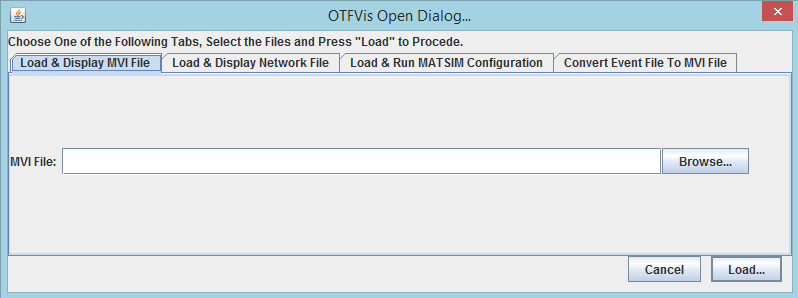
\includegraphics[width=0.95\textwidth, angle=0]{extending/figures/otfvis/image03.png}}%
{}
%---------------------------------------------------------------------

% ============================================================================================
\subsection{Use Cases of \gls{otfvis}}
With the open dialog appearing after starting the vanilla \lstinline|OTVFis| class, the following options arise as shown in Figure~\ref{fig:otfvis_dialog}.
%
\begin{enumerate}\styleEnumerate
	\item Opening a prerecorded \gls{mvi} file,
	\item Opening a network file (for inspection),
	\item Opening a live run of a \gls{matsim} \gls{configfile} (rather memory intensive) or
	\item Converting an event file (plus a given network file) to a movie (\gls{mvi}) file.
\end{enumerate}

Each tab stands for an individual usage. To start a visualization one chooses the appropriate tab, fills the necessary data and finally proceeds by pressing the \lstinline|Load...| button located in the bottom left corner of the window.

In the next sections, an overview is given over the different ways to use \gls{otfvis}.

% ---------------------------------------------------------
\subsubsection{Converting Event Files}
Though the first option tab will be the most commonly used choice for \gls{otfvis}, but the fourth and last option tab is a good starting point for exploring the visualizer: After having successfully run a \gls{matsim} simulation, there will typically be some event files to one's disposal. With any of these event files and a given (matching) network file, a \gls{mvi} file can be created. 
Four items, \ie event, network and movie file names as well as a time period, need to be specified for this tab to execute. 
The last parameter is a time period after which a new sample of the \gls{mobsim}'s state is taken. 
This \gls{mvi}-generation process might be time consuming. For smaller projects it might be an option to choose to display the outcome in the visualizer right away (by checking the box \lstinline|Open mvi afterwards|). 
If the choice is to just convert the events to a \gls{mvi} file, this file can be opened with the first option tab of the visualizers start dialog at any time. 

From the shell this process can be started by giving the event file, the network file and, optionally, the conversion period as input parameters.

% ---------------------------------------------------------
\subsubsection{Network File Loading}
The second option tab will give the opportunity to examine a network file (\eg for errors). 
It will show a rendering of the given network and also, if so chosen in the preferences, the associated network link IDs for each link. 
This option might be helpful for debugging a freshly converted network, or inspect specific regions and connections. Loading and interacting with a network file should be very fast. 

The network file can also be given as the sole parameter to \gls{otfvis} by the shell command.

% ---------------------------------------------------------
\subsubsection{Running a MATSim Configuration}
The third and most advanced option for running \gls{otfvis} is an actual live running \gls{mobsim}, visualized in real time (actually way faster than real time, who has all day to watch tiny cars drive around?). This option includes the possibility to explore the data set and issue queries into the executing \gls{mobsim}. These queries can display an agent's day plan, show all links driven by agent's crossing a particular link of interest, search for a particular link or node by ID or answer whatever user-defined queries there are. We will see later in this chapter how to program own queries, but for the rest of this section we will detail the ``offline'' behavior of \gls{otfvis}. 

It is also feasible to input the \gls{configfile} as a single parameter to \gls{otfvis} by starting it from the shell. \gls{otfvis} will make an educated guess, if the input is a config or a network file.

% ---------------------------------------------------------
\subsubsection{Loading \& Displaying an MVI File}
If the first and default option tab is chosen, an \gls{mvi} file is selected and shown as detailed in next Section~\ref{sec:otfvis-viewing-an-mvi-file}. This is the most common use case for \gls{otfvis}. Same can be achieved by starting \gls{otfvis} from the shell with an \gls{mvi} file as an argument.

% ============================================================================================
\subsection{Viewing an MVI File}
\label{sec:otfvis-viewing-an-mvi-file}
An example of this is illustrated in Figure~\ref{fig:OTFVisRunning}. On the top left of the application one finds buttons for controlling the playback of the file. A short summary of the functionality is given in Table~\ref{tab:otfvis-buttonbar}.

This buttonbar is followed by a text field into which the wanted time can be written for an instant jump. In an \gls{mvi} file jumping forward and backward in time is possible, whereas in the live simulation case going back in time is omitted.

Another way of iterating through the animation is to grab the time slider at the bottom of the application and drag it. 
On the left side of the slider are opening and closing bracket symbols. 
By clicking them one can set the start respectively the end time of a time loop to the actual time step given. 
Therefore, it is possible to restrict playback to a certain space of time.

%---------------------------------------------------------------------
\createfigure%
{Displaying an MVI file}%
{Displaying an MVI file}%
{\label{fig:OTFVisRunning}}%
{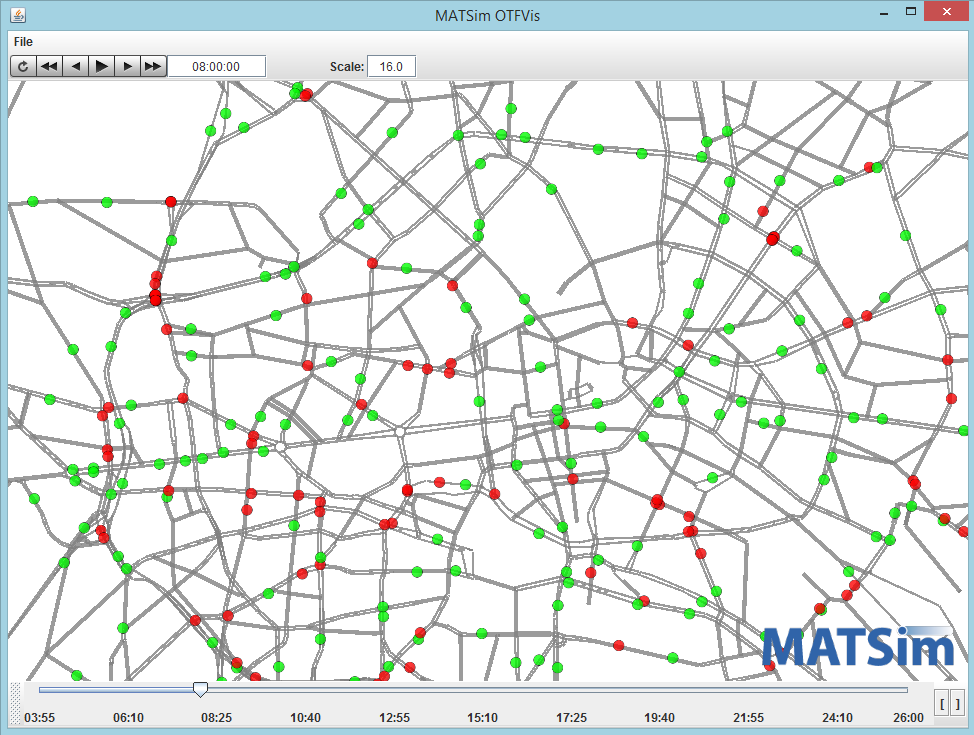
\includegraphics[width=0.95\textwidth, angle=0]{extending/figures/otfvis/image06.png}}%
{}
%---------------------------------------------------------------------
%---------------------------------------------------------------------
\createtable%
{OTFVis Buttonbar}%
{OTFVis Buttonbar}%
{\label{tab:otfvis-buttonbar}}%
{%
  \begin{tabular}[c]{|m{1cm}|m{6cm}|}
    \hline
    \textbf{Icon}  & \textbf{Function} \\
    \hline
		\raisebox{-.17\height}{
\includegraphics[width=0.03\textwidth]{extending/figures/otfvis/image00.png}} & Reset - set time to the start time\\
		\hline
		\raisebox{-.17\height}{
\includegraphics[width=0.03\textwidth]{extending/figures/otfvis/image01.png}} & Large step back\\
		\hline
		\raisebox{-.17\height}{
\includegraphics[width=0.03\textwidth]{extending/figures/otfvis/image09.png}} & Small step back\\
		\hline
		\raisebox{-.17\height}{
\includegraphics[width=0.03\textwidth]{extending/figures/otfvis/image05.png}} & Play \\
		\hline
		\raisebox{-.17\height}{
\includegraphics[width=0.03\textwidth]{extending/figures/otfvis/image07.png}} & Pause \\
		\hline
		\raisebox{-.17\height}{
\includegraphics[width=0.03\textwidth]{extending/figures/otfvis/image02.png}} & Small step forward \\
		\hline
		\raisebox{-.17\height}{
\includegraphics[width=0.03\textwidth]{extending/figures/otfvis/image10.png}} & Large step forward \\
		\hline
  \end{tabular}
}%
{}
%---------------------------------------------------------------------

% ============================================================================================
\subsection{General Interaction with the Main Screen}
Regardless which option for loading data was chosen, the interaction with the main display area is the same.
%
\begin{description}\styleDescription
\item[Right button drag:] Extend a rectangle for zooming into the view. Releasing the button will execute a zoom, so the chosen rectangle will best fit the screen.
\item[Middle-Mouse-drag:] Pan (translate) the screen.
\item[Right-Mouse-Click:] Show a context menu (for now only with the option to save the view settings)
\end{description}

% ============================================================================================
\subsection{User Interaction in the Live Mobsim}
When started as a live simulation, \gls{otfvis} will present a different appearance as shown in Figure~\ref{fig:OTFVisLive}. 
First, the controls over the flow of the simulation's view are a restricted subset of the ones used in \gls{mvi} playback. 
There is no possibility to reset the simulation or to rewind it. 
One can still make small or large steps forward. 
A new option is given by the \lstinline|synch| checkbox. 
It determines whether the \gls{mobsim} will stop for each frame the \gls{otfvis} renders or run independently. 
Usually the \lstinline|un-synched| version will proceed faster, as the \gls{otfvis} output is restricted to a default of about 30\,frames/updates per second and a small \gls{mobsim}'s simulation speed will be a magnitude higher. 
Also, the time consuming generation of visualization data will only be necessary for a smaller fraction of the simulation. 
How long the \gls{otfvis} pauses between frames can be configured in the preferences dialog.

Apart from the reduced control set, there is another UI element new to this \gls{otfvis} option. 
At the bottom of the screen, the scrubbar/time line element is replaced by a ``query'' bar. 
It is possible to code ``queries'' into the \gls{mobsim}, answering questions about the inner state of it. 
As the simulation is actually happening, all information necessary to run it is available for output. 
This is a clear superset of the information available in the event files and therefore in the \gls{mvi} files. 
This rich information infrastructure can be queried and visualized in many ways. 
In the next session an example for a query is given.

%---------------------------------------------------------------------
\createfigure%
{Live mode}%
{Live mode}%
{\label{fig:OTFVisLive}}%
{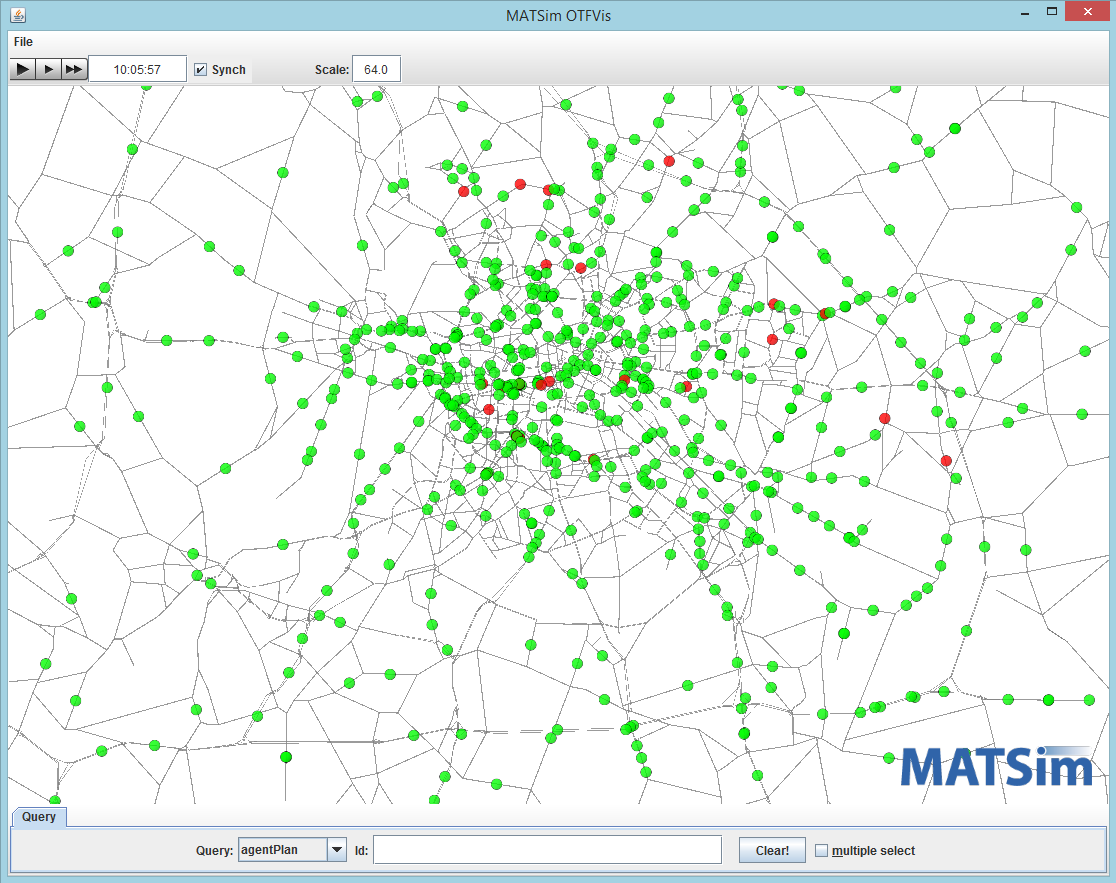
\includegraphics[width=0.95\textwidth, angle=0]{extending/figures/otfvis/image04.png}}%
{}
%---------------------------------------------------------------------

% ============================================================================================
\subsection{Running a Query in \gls{otfvis} Real Time Data}
From the dropdown box one can choose the different query types. 
Often, additional input is necessary. This can be done either by the text field next to it or, more often, by clicking into the network. 
To give an example, with \lstinline|agent query| selected, a click onto any agent's symbol will give a visualization of this particular agent's day plan. 
This is shown in Figure~\ref{fig:OTFVisAgent}. There are other pre-defined queries. 
These queries are rather project-oriented, so defining own queries will be most likely necessary to make best use of this option. 
In the second part of this chapter we will look into defining own queries.

%---------------------------------------------------------------------
\createfigure%
{Queries}%
{Queries}%
{\label{fig:OTFVisAgent}}%
{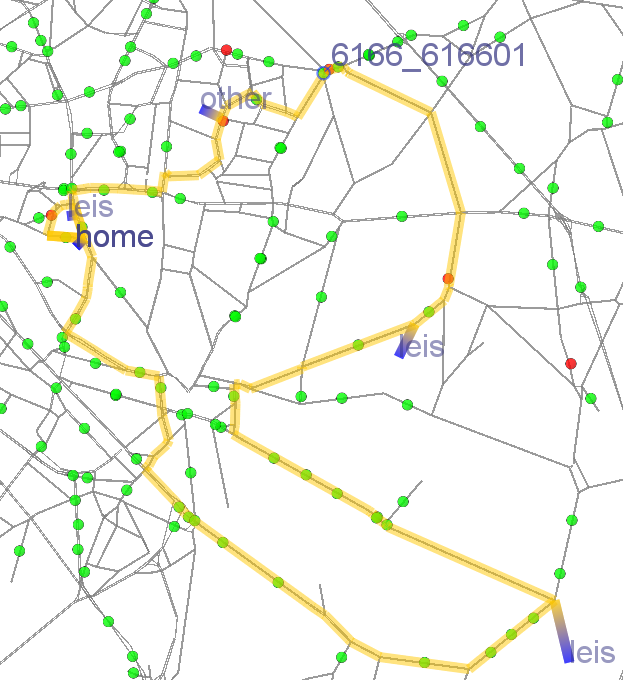
\includegraphics[width=0.35\textwidth, angle=0]{extending/figures/otfvis/image08.png}}%
{}
%---------------------------------------------------------------------

% ##################################################################################################################
\section{Extending \gls{otfvis}}
Being open source, the \gls{otfvis} is a good starting point for customizing visualizations of mobsim runs. 
\gls{otfvis} has been written in \gls{java}, but it heavily depends on the \gls{jogl} \gls{java} library.% (link). 
\gls{jogl} is a very thin layer within the hardware driver of the \gls{os}, meaning it will have \gls{os}-specific, native dependencies. 
These should be taken care of by the maven-dependency management, but nonetheless should be had in mind when developing for \gls{otfvis}. 
The displaying parts of \gls{otfvis} are based on \gls{opengl}. 
Therefore, it will be necessary to have knowledge of \gls{opengl} to write new ways of displaying data. 
In the following sections, it will be examined how data is computed inside the \gls{otfvis} and how this can be extended.

% ============================================================================================
\subsection{Design Principles of \gls{otfvis}}
The overall goal for designing \gls{otfvis} was to have an easy to extend, fast visualizer capable of handling huge amounts of data. 
The specific design goals for the visualizer were:
%
\begin{itemize}
\item Abstract data source (data collection) from data display (visualization)
\item Easy to extend with own data types
\item Simulation can be run locally on desktop computer
\item Reduce the amount of sent data to a minimum
\item Visualization can connect to running simulation (on-the-fly)
\item Minimally-invasive to existing \gls{matsim} code
\item Fast enough for large scenarios
\item Visualization can read from post-mortem dump (\gls{mvi} file)
\item Take advantage of hardware support for drawing
\end{itemize}
%
\gls{matsim} runs can easily engage millions of agents traveling a network. To make a visualization of these large data sets feasible two measures have been taken. A quad tree structure was implemented to ensure only the smallest set of data necessary to display the visible sector of the network is transferred. The quad tree is a simple data structure to aggregate spatial data and retrieve parts of it in a timely manner for real time visualization. Apart from data structures, hardware is also used to speed up displaying the simulation. \gls{opengl} is a platform independent \gls{api} to interface graphics hardware, namely the 3D acceleration chips implemented in every contemporary computer. With the aid of 3D graphics hardware, even millions of agents can be displayed in real time. Other measures were taken to segregate data extraction from data visualization, like the reader/writer pairs presented in the next section.

% ============================================================================================
\subsection{Readers and Writers}
\gls{otfvis} was designed to have minimal dependencies on the \gls{mobsim} used. Data formats applied within the \gls{mobsim} should be abstracted from data used in \gls{otfvis}. Therefore, any data passed to the visualizer will have to run through some stages of abstraction.

The first stage is a writer-reader pair, responsible to transfer a certain set of data to the \gls{otfvis}. The writer will understand the data format of the hosting \gls{mobsim} and convert it to simple data types like float or string values. A set of these writers will be called after each mobsim step to accumulate data. These writers all use a joint byte buffer to aggregate the data. This array of bytes is then send to the visualizer, which in the original design could be run anywhere in your network.

For each writer, there has to be a sibling-reader class, responsible to read back the extracted data from the byte buffer. 
It is crucial to enforce that these pairs work synchronously. Most Writer/Reader-pairs are being implemented in the same class, since having the source-code at the same place reduces errors in the synchronization.

Apparently, it can be necessary or useful to have different ways to visualize data on the \gls{otfvis} frontend. Therefore, the actual readers are not responsible for the drawing of a certain data set. A third kind of class is responsible to do that, the drawer classes.

% ============================================================================================
\subsection{Visualization of the Data}
The reader objects in the quad tree will generate separate drawer objects for displaying ``their'' information and add these to another data structure called \lstinline|SceneGraph| responsible for the actual drawing onto an \gls{opengl} canvas. 
Displaying data in an interactive application will make re-draws of the display necessary due to a variety of reasons (\eg displaying menus, animations, zooming, panning and other user interactions). 
Not all of these changes introduce new data from the \gls{mobsim}. 
Zooming into the network will not imply reading data from the \gls{mobsim}, whilst panning the view most certainly will. 
When no new data is needed, the scene graph is capable to handle all operations, no reader/writer class will be accessed and displaying is solely done with existing drawers. 
On the other hand, if new data is in demand, the scene graph will be ``invalidated'' (a term lent from the \gls{opengl} community) thus the graph will be dismissed and all relevant readers will be asked for new drawer objects representing the actual view. The scene graph is mainly a list of drawer objects. As an extra structuring unit, these drawers can be sent into different layers, to render them more effectively.

% ============================================================================================
\subsection{Layers}
To minimize data being send to what is actually necessary for drawing the particular area visible in the viewport, writers should minimize the data packets, so the quad tree can make a spatial reduction of the data. This does not meet very well with \gls{opengl} (or any graphics \gls{api}). The \gls{api} wants data to be most accumulated, to optimize output through the graphics pipeline of the underlying hardware. 
Think of an assembly line vs. handcrafted item: whenever the flow of data is interrupted, the assembly line stalls and graphics performance derogates. 
To ease this issue, ``layers'' have been introduced to \gls{otfvis}. 
Any drawer (responsible for a bit of information) can be assigned to a layer. 
These layers will finally be called to draw the screen's content. 
It is up to the layer to possibly optimize the execution of the drawers. 
For example, a network layer might store all network info from the drawer into one array or display list to optimize drawing of the network (often in \gls{opengl} it is advisable to rather let the hardware decide what to draw. 
It might be faster, if the complete data can reside in graphics hardware memory, rather than to transfer the reduced set of information every frame). There are three layers predefined in \gls{otfvis}. 
The \lstinline|networkLayer| contains the static street net, the \lstinline|agentLayer| contains the actual dynamic agents and a third layer, the \lstinline|miscellaneousLayer|, will contain additional data.

% ============================================================================================
\subsection{Patching the Connections}
In total there are four basic elements involved in the visualization: writers, readers, drawers and layers. 
To configure how the first two work together, an additional class takes responsibility: \lstinline|OTFConnectionManager|.

This class maps several routes for the information coming from the \gls{mobsim}, building a chain of responsibility. 
Each data item starts at a link in our network. 
An \lstinline|OTFDataWriter| object is responsible to extract the wanted data from the link and write it into a \lstinline|ByteBuffer|. 
Complementing this, an associated \lstinline|OTFDataReader| is needed to retrieve the data from the buffer. 
This item will also be responsible to add a drawable item derived from the class \lstinline|OTFGLAbstractDrawable| to the scene graph representing the actual screen content. 
The connection between these items is made by adding entries into the \lstinline|OTFConnectionManager| with calls to \lstinline|OTFConnectionManager.connectLinkToWriter(OTFDataWriter)| 
and \lstinline|OTFConnectionManager.connectLinkToWriter(OTFDataWriter, OTFDataReader)| respectively.
 
Example (from the \lstinline|OTFClientLive.java|):

\lstinline|conMan.connectLinkToWriter(OTFLinkAgentsHandler.Writer.class);| \\
\lstinline|conMan.connectWriterToReader(OTFLinkAgentsHandler.Writer.class,|
\lstinline|OTFLinkAgentsHandler.class);|

% ============================================================================================
\subsection{Sending the Data}
The class \lstinline|OTFLinkAgentsHandler| should give a good example how to extract, send, receive and display data in the \gls{otfvis} context. The method \lstinline|invalidate| is called whenever the actual scene graph has been dismissed and needs to be rebuild. 
In this case, a valid representation for the state of this object should be added to the new scene graph. 
This also means that for drawing the actual scene, no additional reading will take place. 
Only if there is a change in the data visible, this update is triggered.

% ============================================================================================
\subsection{Performance Considerations}
When implementing new ways to visualize data the following guidelines should be taken into consideration.

If the data is spatially distributed over the whole network and is updated frequently, an \lstinline|OTFDataWriter/Reader| pair should be considered. 
It will reduce an updating of the data to times when the data is actually visible, not creating, transporting or drawing the data otherwise. If a fraction of the data needs to be transferred only once---because it is static over the time of the simulation---it can be sent with the \lstinline|writeConstData()| method; otherwise using \lstinline|writeDynData()| is advised. 
If the data is sparse and little information is transmitted or it has no discernible spatial cohesion, it might be simpler to just add it to the server quad tree as additional data with a call to \lstinline|OTFServerQuadTree.addAdditionalElement()|. 

% ============================================================================================
\subsection{Sending Live Data}
The flow of data within \gls{otfvis} is a strict one way affair at most times. 
Except for one important issue: Sending queries into the simulation. In case of a live simulation run visualized with the help of the \lstinline|OTFVisLiveClient| class, queries can be send into the simulation. 
Again, this process is threefold in terms of the methods involved. Queries will be realized through an object derived from the abstract class \lstinline|AbstractQuery|. Such an object implements several methods that will be used as callback over the lifetime of the query.

First, a new query is sent to the server and the method \lstinline|installQuery()| is called. 
In this method, all relevant parts (network, population, events) of the simulation run can be accessed and data can be collected. 
The visualizer framework will later repeatedly call the \lstinline|result()| method, to retrieve an \lstinline|OTFQueryResult| object. 
This needs to implement a \lstinline|draw()| method, to visualize the results in the given screen context. 
If the result indicates \lstinline|isAlive()|, the \lstinline|query()| method of the \lstinline|AbstractQuery|-derived object will be called each frame, otherwise it will be called only once.

% ##################################################################################################################








